\title{A harebrained attempt to collect during peak snowshoe hare}

\subtitle{\doi{10.7299/X7R211Q0}}

\author{by Adam Haberski}

\maketitle

My study site looked like the aftermath of a hurricane. Pitfall traps and bee bowls had been torn up from the ground and thrown far from where I had carefully set them two weeks before. Any specimens they might have contained were long gone. I dropped my heavy backpack, sat down in the center of the wreckage, and made an entry into my field notebook. “19 July 2018: Total destruction. Again.”

I was well into the third field season of my thesis work studying alpine arthropods in Denali National Park \& Preserve, Alaska. Working in Denali had been a dream come true. The scenery and wildlife viewing are unparalleled. I was joined by my advisor, Derek Sikes, the park entomologist Jessica Rykken, and her interns Felix and Amber. The work wasn’t always easy, and we had overcome challenges---incessant rain, curious bears, indignant tourists, and navigating bus traffic along the precipitous Polychrome Pass to name a few---but we were a crack team and it was the kind of  “type two fun” that I enjoy. But with each destroyed sample, my excitement was fading into frustration. The culprits, of all things, were snowshoe hares (Figure \ref{hare}).

Snowshoe hares (\textit{Lepus americanus}) are normally innocuous herbivores, but something about the site of plastic pitfall traps excites them into a frenzy. Their usual modus operandi is to grip the rim of the trap between their teeth and toss it disdainfully over their heads. Other times, they will dig under a bee bowl and chew a small hole in the bottom to drain the liquid without disturbing the bowl. A family of hares can reduce a study site to plastic splinters in a matter of hours. I set up a motion sensing camera to record them in the act. The mischief began only 20 minutes after I left the area and didn’t stop until the camera’s memory card was full. I combined the images into a time-lapse video (\url{https://youtu.be/d1hfV4lYR7E}). It resembles a scene from \textit{Night of the Lepus} or \textit{Monty Python and the Holy Grail}.

Open any ecology textbook and you will find a graph of the hare population cycle. Hare populations rise and fall every ten years or so, followed closely by their predator, the Canada Lynx (\textit{Lynx canadensis}) \citep{Krebsetal2001}. In 2018, the Denali population was approaching its peak. It was evident in the evenings when they gathered along the Park Road in the hundreds. At that density, they become non-demonic intrusion incarnate. I feared for my thesis. 

\begin{figure}[H]
\begin{center}
\vspace{2mm}
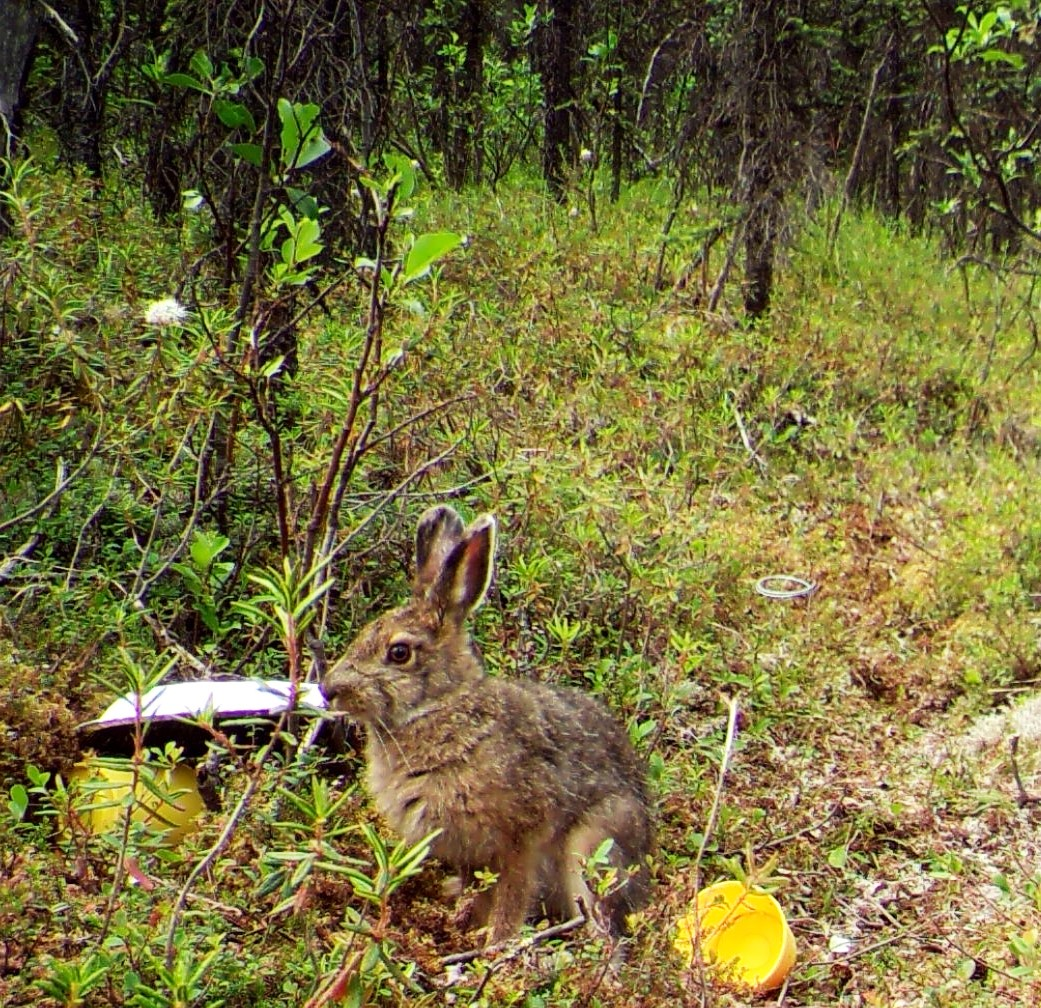
\includegraphics[width=\textwidth]{img/hare.jpg}
\caption{An audacious snowshoe hare (\textit{Lepus americanus)} caught in the act of vandalizing precious entomological equipment.}
\label{hare}
\end{center}
\end{figure}  

We na\"{i}vely believed that, as resourceful scientists, we could outsmart the hares. Our first attempt was to add a bittering agent to the traps’ liquid preservative. Denatonium benzoate is the most bitter chemical compound known, with a bitterness threshold of only 0.01 parts per million. A single grain will leave a bad taste in your mouth for days (I can speak from experience). We mixed a teaspoon into every gallon of preservative. Jessica went as far as to spray denatonium solution on the outside of her bee bowls. One taste should have sent the hares running. Unfortunately, we were unaware that animals perceive bitterness differently than we do. Rodents, the sister order to hares, are 100,000 times less sensitive to denatonium than humans \citep{Franketal2004}. 

The next step was mechanic exclusion. I built chicken wire cages and secured them over the traps with 8-inch steel spikes (Figure \ref{hare_cage}). The hares dug below the spikes and flipped the cages aside with the same contempt they showed my pitfall traps. By that time, the season was nearly over, and our spirits were broken.

\begin{figure}[H]
\begin{center}
\vspace{2mm}
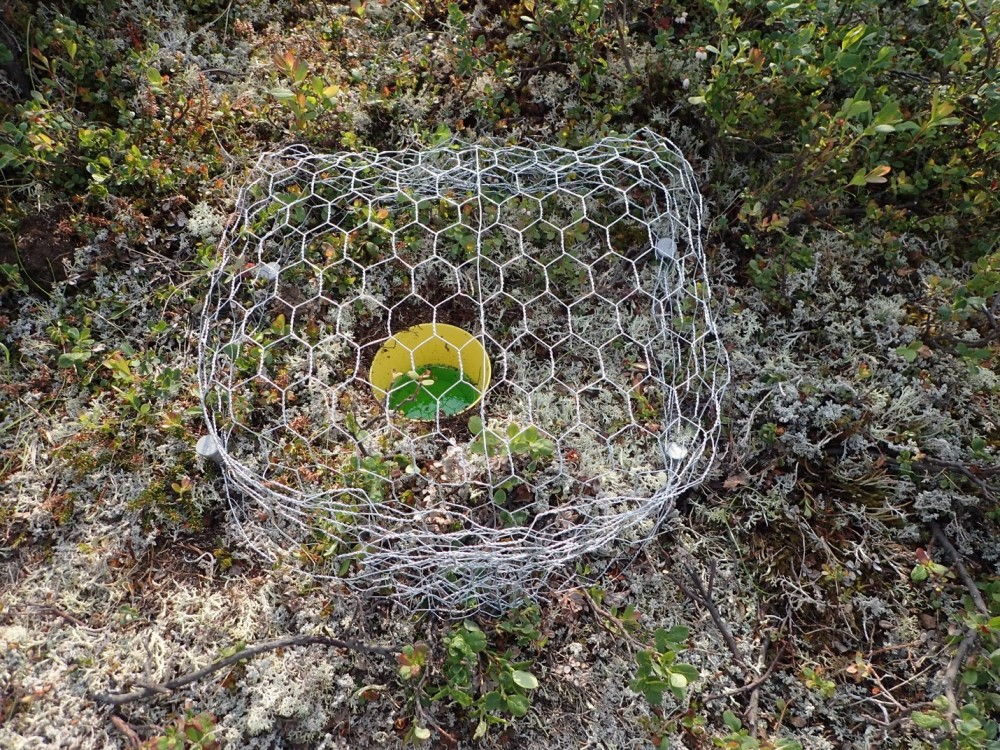
\includegraphics[width=\textwidth]{img/hare_cage.jpg}
\caption{This chicken wire cage proved ineffective at excluding hares and preserving my pride.}
\label{hare_cage}
\end{center}
\end{figure} 

In the end, the only solution was the natural ebb of the hare population cycle. I drove the Park Road one evening in 2019 and the throngs of hare were gone. The park was once again safe for entomologists. The final toll was 30\% of my traps tipped, chewed, lost, or otherwise destroyed, but it was enough to finish my thesis. Still, I fear for the future. This project was envisioned as the beginning of a long-term research project to monitor arthropods’ response to climate change. The original schedule called for re-sampling every ten years, perfectly coinciding with the next peak in snowshoe hare.

%\bibliography{hares}

\begin{thebibliography}{2}
\expandafter\ifx\csname natexlab\endcsname\relax\def\natexlab#1{#1}\fi
\expandafter\ifx\csname url\endcsname\relax
  \def\url#1{{\tt #1}}\fi
\expandafter\ifx\csname urlprefix\endcsname\relax\def\urlprefix{{\small URL}
  }\fi

\bibitem[{Frank et~al.(2004)Frank, Bouverat, MacKinnon, and
  Hettinger}]{Franketal2004}
Frank, M.~E., B.~P. Bouverat, B.~I. MacKinnon, and T.~P. Hettinger.
\newblock 2004.
\newblock The distinctiveness of ionic and nonionic bitter stimuli.
\newblock Physiology \& Behavior {\bfseries 80}:421--431.
\newblock \doi{10.1016/j.physbeh.2003.09.009},
  \urlprefix\url{http://www.sciencedirect.com/science/article/pii/S0031938403003007}.

\bibitem[{Krebs et~al.(2001)Krebs, Boonstra, Boutin, and
  Sinclair}]{Krebsetal2001}
Krebs, C.~J., R.~Boonstra, S.~Boutin, and A.~Sinclair.
\newblock 2001.
\newblock {What Drives the 10-year cycle of snowshoe hares?: {The} ten-year
  cycle of snowshoe hares---one of the most striking features of the boreal
  forest---is a product of the interaction between predation and food supplies,
  as large-scale experiments in the {Yukon} have demonstrated}.
\newblock BioScience {\bfseries 51}:25--35.
\newblock \doi{10.1641/0006-3568(2001)051[0025:WDTYCO]2.0.CO;2}.

\end{thebibliography}
